%%%%%%%%%%%%%%%%%%%%%%%%%%%%%%%%%%%%%%%%%%%%%%%%%%%%%%%%

\documentclass[12pt,a4paper]{article}% 文档格式
\usepackage{ctex,hyperref}% 输出汉字
\usepackage{times}% 英文使用Times New Roman
%%%%%%%%%%%%%%%%%%%%%%%%%%%%%%%%%%%%%%%%%%%%%%%%%%%%%%%%
\title{\fontsize{18pt}{27pt}\selectfont% 小四字号，1.5倍行距
	{\heiti% 黑体 
		Life Lab：AI Agent 社会实验平台\\% 题目
		设计文档}}%
%%%%%%%%%%%%%%%%%%%%%%%%%%%%%%%%%%%%%%%%%%%%%%%%%%%%%%%%
\author{\fontsize{12pt}{18pt}\selectfont\fangsong
	赵俊宇~~刘福康~~岳雨婷\\[3pt]
	\fontsize{10.5pt}{15.75pt}\selectfont\fangsong
	(中国科学技术大学~~~信息科学技术学院)}
%%%%%%%%%%%%%%%%%%%%%%%%%%%%%%%%%%%%%%%%%%%%%%%%%%%%%%%%
\date{}% 日期（避免生成日期）
%%%%%%%%%%%%%%%%%%%%%%%%%%%%%%%%%%%%%%%%%%%%%%%%%%%%%%%%
\usepackage{amsmath,amsfonts,amssymb}% 为公式输入创造条件的宏包
%%%%%%%%%%%%%%%%%%%%%%%%%%%%%%%%%%%%%%%%%%%%%%%%%%%%%%%%
\usepackage{graphicx}% 图片插入宏包
\usepackage{subfig}% 并排子图
\usepackage{subcaption}
\usepackage{float}% 浮动环境，用于调整图片位置
\usepackage[export]{adjustbox}% 防止过宽的图片
\usepackage{multirow}
\usepackage[table,xcdraw]{xcolor}
\usepackage{colortbl}
%%%%%%%%%%%%%%%%%%%%%%%%%%%%%%%%%%%%%%%%%%%%%%%%%%%%%%%%
\usepackage{bibentry}
\usepackage{natbib}% 以上2个为参考文献宏包
\setcitestyle{numbers,square}
%%%%%%%%%%%%%%%%%%%%%%%%%%%%%%%%%%%%%%%%%%%%%%%%%%%%%%%%
\usepackage{abstract}% 两栏文档，一栏摘要及关键字宏包
\renewcommand{\abstracttextfont}{\fangsong}% 摘要内容字体为仿宋
\renewcommand{\abstractname}{\textbf{摘\quad 要}}% 更改摘要二字的样式
%%%%%%%%%%%%%%%%%%%%%%%%%%%%%%%%%%%%%%%%%%%%%%%%%%%%%%%%
\usepackage{xcolor}% 字体颜色宏包
\newcommand{\red}[1]{\textcolor[rgb]{1.00,0.00,0.00}{#1}}
\newcommand{\blue}[1]{\textcolor[rgb]{0.00,0.00,1.00}{#1}}
\newcommand{\green}[1]{\textcolor[rgb]{0.00,1.00,0.00}{#1}}
\newcommand{\darkblue}[1]
{\textcolor[rgb]{0.00,0.00,0.50}{#1}}
\newcommand{\darkgreen}[1]
{\textcolor[rgb]{0.00,0.37,0.00}{#1}}
\newcommand{\darkred}[1]{\textcolor[rgb]{0.60,0.00,0.00}{#1}}
\newcommand{\brown}[1]{\textcolor[rgb]{0.50,0.30,0.00}{#1}}
\newcommand{\purple}[1]{\textcolor[rgb]{0.50,0.00,0.50}{#1}}% 为使用方便而编辑的新指令
%%%%%%%%%%%%%%%%%%%%%%%%%%%%%%%%%%%%%%%%%%%%%%%%%%%%%%%%
\usepackage{url}% 超链接
\usepackage{bm}% 加粗部分公式
\usepackage{booktabs}
\usepackage{longtable}% 长表格
\usepackage{supertabular}% 跨页表格
\usepackage{algorithm}
\usepackage{algorithmic}
\usepackage{changepage}% 换页

\usepackage{listings}
\lstset{
    basicstyle=\ttfamily\small,
    numbers=left,
    numberstyle=\tiny\color{gray},
    stepnumber=1,
    backgroundcolor=\color{gray!8},
    frame=single,
    rulecolor=\color{black!30},
    tabsize=2,
    breaklines=true,
    captionpos=b,
    showstringspaces=false,
    keywordstyle=\color{blue},
    commentstyle=\color{green!50!black},
    stringstyle=\color{purple},
    escapeinside={(*@}{@*)},
    columns=fullflexible,
    extendedchars=true,
    inputencoding=utf8
}
%%%%%%%%%%%%%%%%%%%%%%%%%%%%%%%%%%%%%%%%%%%%%%%%%%%%%%%%
\usepackage{enumerate}% 短编号
\usepackage{caption}% 设置标题
\captionsetup[figure]{name=\fontsize{10pt}{15pt}\selectfont Figure}% 设置图片编号头
\captionsetup[table]{name=\fontsize{10pt}{15pt}\selectfont Table}% 设置表格编号头
%%%%%%%%%%%%%%%%%%%%%%%%%%%%%%%%%%%%%%%%%%%%%%%%%%%%%%%%
\usepackage{indentfirst}% 中文首行缩进
\usepackage[left=2.50cm,right=2.50cm,top=2.80cm,bottom=2.50cm]{geometry}% 页边距设置
\renewcommand{\baselinestretch}{1.5}% 定义行间距（1.5）
%%%%%%%%%%%%%%%%%%%%%%%%%%%%%%%%%%%%%%%%%%%%%%%%%%%%%%%%
\usepackage{tikz} % TikZ 绘图（架构图）
\usetikzlibrary{arrows.meta, positioning, calc}
\usepackage{fancyhdr} %设置全文页眉、页脚的格式
\pagestyle{fancy}
\hypersetup{colorlinks=true,linkcolor=black}% 去除引用红框，改变颜色
%%%%%%%%%%%%%%%%%%%%%%%%%%%%%%%%%%%%%%%%%%%%%%%%%%%%%%%%
% ── 架构图颜色定义 ──
\definecolor{clrGreen}{HTML}{2E7D32}\definecolor{clrGreenBg}{HTML}{E8F5E9}
\definecolor{clrBlue}{HTML}{1565C0}\definecolor{clrBlueBg}{HTML}{E3F2FD}
\definecolor{clrOrange}{HTML}{E65100}\definecolor{clrOrangeBg}{HTML}{FFF3E0}
\definecolor{clrPurple}{HTML}{6A1B9A}\definecolor{clrPurpleBg}{HTML}{F3E5F5}
\definecolor{clrRed}{HTML}{C62828}\definecolor{clrRedBg}{HTML}{FFEBEE}
\definecolor{clrArrow}{HTML}{546E7A}\definecolor{clrTitle}{HTML}{1A237E}
%%%%%%%%%%%%%%%%%%%%%%%%%%%%%%%%%%%%%%%%%%%%%%%%%%%%%%%%

\begin{document}
	\graphicspath{{E:/latex/documents/xinliarticle}{E:/download}}
\begin{figure}[t]
	\includegraphics[width=0.4\textwidth]{7-1401291J307.png}
\end{figure}
	\maketitle 
	
	\begin{abstract}
		\fangsong 本文档描述 AI Agent 社会实验平台 Life Lab 的系统设计。平台采取\textbf{"快慢结合"}、多链路并行的设计思想：关键词匹配能快速给出初步判断，但不够准确；LLM 深度评估需要数秒，但更可靠。两条独立路径互相保险，对抗 LLM 可能产生的错误。在此哲学之上，平台实现了三项核心能力：\textbf{人格驱动的社会涌现}（MBTI 人格直接决定 Agent 怎么移动、怎么社交、怎么产生情绪）、\textbf{可信赖的多 Agent 协作}（DAG 管道编排 + 程序直接验证每一步是否真正执行）和\textbf{可解释的行为评测}（六个维度打分 + 信息论量化行为一致性 + 逐维度诊断证据链）。本文档重点阐述 M9--M12 四个进阶模块的设计决策，揭示从基础模块到进阶能力的生长脉络，并说明大模型应用方式与调试优化策略。
	\end{abstract}
	
	\noindent\fbox{\parbox{0.95\textwidth}{
	\textbf{\heiti 核心亮点}
	\begin{itemize}
		\item \textbf{"多链路设计"}：关键词匹配 1ms 出结果，LLM 深度评估数秒但更可靠，双路径互保
		\item \textbf{人格直接决定行为}：MBTI 等可直接驱动对话/移动/情绪三维度，从"说什么"到"怎么走"全链路一致
		\item \textbf{DAG 管道编排 + 程序直接验证交付}：支持 Loop/Branch 控制流，算式直接算一遍、工具记录直接查一遍，不依赖 LLM 判断
		\item \textbf{用信息论量化行为} + 跨任务鲁棒性 + 逐维度诊断，确保行为评测从定性走向定量
		\item \textbf{多模型集成}：支持 DeepSeek / GLM / OpenAI，统一 OpenAI 兼容 API，内置超时重试与降级兜底
		\item \textbf{20 页面} + Phaser 3 + 图形化管线编辑器，保障系统完整度与工程成熟度
	\end{itemize}
	}}
	\vspace{0.5em}
	
	\begin{adjustwidth}{1.06cm}{1.06cm}
		\fontsize{10.5pt}{15.75pt}\selectfont{\heiti{关键词：}\fangsong{AI Agent；系统架构；人格建模；多智能体协作；行为指纹；管道编排}}\\
	\end{adjustwidth}

\newpage
\tableofcontents
	
\newpage

%% ============================================================
\section{引言}
%% ============================================================

\subsection{设计目标}

\begin{enumerate}
	\item \textbf{人格真实性}：Agent 行为应与其人格参数保持一致，不同人格在相同场景下表现出可辨识的行为差异。
	\item \textbf{可扩展性}：引擎层通过 Mixin 模式组合能力，新功能添加不影响既有系统。
	\item \textbf{实时性}：通过 SSE 实现毫秒级事件推送，前端实时渲染 Agent 思维流和行为。
	\item \textbf{鲁棒性}：LLM 调用具备超时、重试和降级机制，关键路径均有规则兜底方案。
	\item \textbf{可信赖性}：多 Agent 协作的每一步交付由程序直接验证，不依赖 LLM 判断，确保任务执行的可审计性。
\end{enumerate}

\subsection{设计原则}

\begin{itemize}
	\item \textbf{引擎与 API 分离}：核心逻辑封装在引擎层（engines），API 层仅负责路由和参数校验。
	\item \textbf{LLM 优先 + 规则兜底}：关键决策优先使用 LLM，不可用时降级为规则引擎。
	\item \textbf{多链路设计}：关键词匹配能在 1ms 内给出初步判断（每 tick，$O(n)$），但不够准确；LLM 深度评估需要数秒，但更可靠。两条路径\textbf{独立运行、互为保险}，快的保证实时性，慢的保证准确性。形式化地，最终判定为 $D = D_{fast} \oplus D_{slow}$，任一路径异常即触发告警。这一模式在关系评估、任务分解、交付验收等多个模块中反复出现，是平台的核心工程哲学。
\end{itemize}

\subsection{竞品对比与设计定位}

\begin{table}[H]
	\centering
	\begin{tabular}{lcccc}
		\toprule
		& \textbf{人格建模} & \textbf{行为评测} & \textbf{游戏化场景} & \textbf{交付验证} \\
		\midrule
		AutoGen / CrewAI & \checkmark（基础） & --- & --- & --- \\
		LangGraph & --- & --- & \checkmark（静态可视化） & --- \\
		AgentBench & --- & \checkmark（黑箱评分） & --- & --- \\
		\textbf{Life Lab} & \checkmark & \checkmark（可解释） & \checkmark（实时交互） & \checkmark \\
		\bottomrule
	\end{tabular}
\end{table}

现有 Agent 框架各有侧重，但均缺乏"人格--行为--评测"的完整链路。Life Lab 的独特定位是：\textbf{不仅是 Agent 编排工具，更是 Agent 社会实验平台}。

%% ============================================================
\section{系统总体架构}
%% ============================================================

系统模块按能力由浅到深分为三层，如图 \ref{fig:arch} 所示：

\begin{figure}[H]
	\centering
	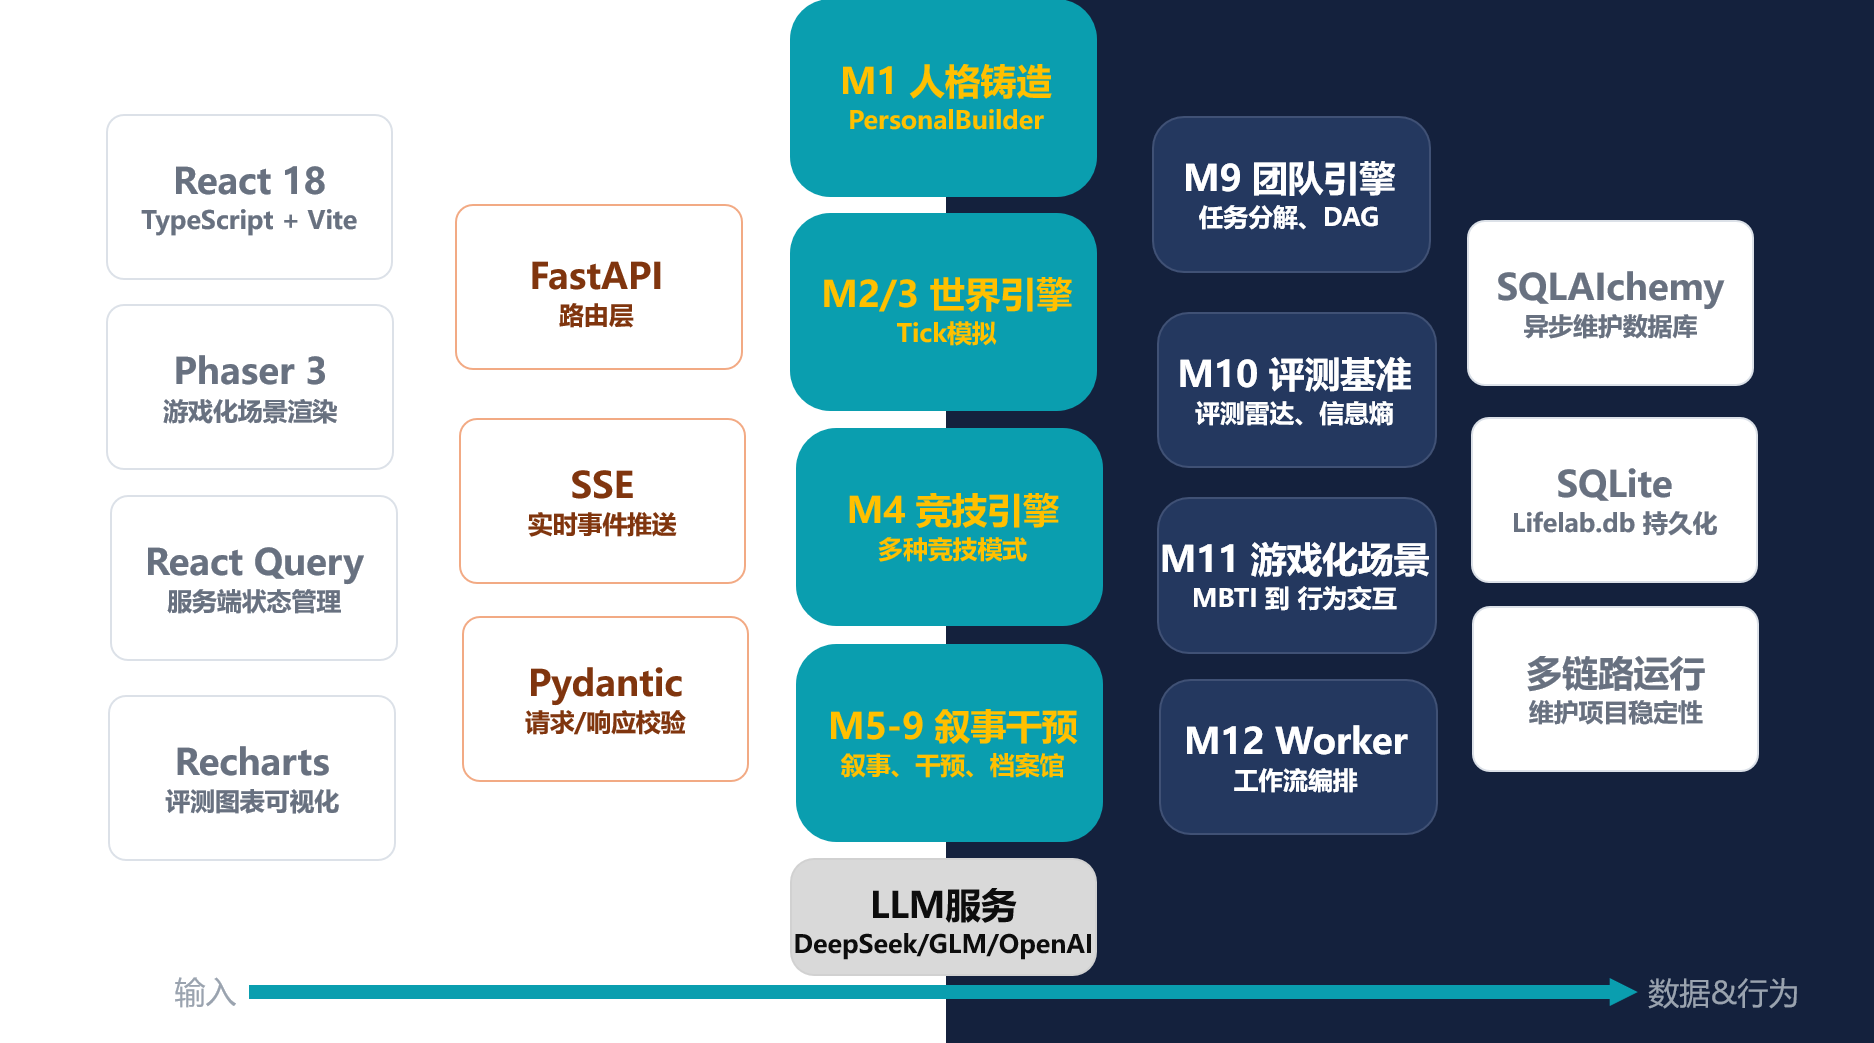
\includegraphics[width=0.95\textwidth]{arch_tech copy.png}
	\caption{Life Lab 系统技术架构图：表现层（React + Phaser 3）$\to$ 接口层（FastAPI + SSE）$\to$ 引擎层（8 大引擎）$\to$ 数据层（SQLAlchemy + SQLite）。LLM 服务通过 OpenAI 兼容 API 接入。}
	\label{fig:arch}
\end{figure}

\begin{enumerate}
	\item \textbf{表现层}：React + TypeScript + TailwindCSS + Phaser 3，通过 React Query 管理服务端状态，SSE 接收实时事件。
	\item \textbf{接口层}：FastAPI 路由层，提供 RESTful API 和 SSE 端点。
	\item \textbf{引擎层}：persona/、agent\_factory/、world/、narrative/、arena/、team/、bench/、worker/ 八大引擎，通过 Mixin 模式组合能力。
	\item \textbf{数据层}：Pydantic 模型 + SQLAlchemy 异步 ORM + SQLite/aiosqlite。
\end{enumerate}

八大引擎分别负责不同的核心职责：persona/ 负责自然语言铸造人格，agent\_factory/ 负责 Agent 实例化和记忆管理，world/ 负责世界模拟和关系演化，narrative/ 负责 9 种文体叙事生成，arena/ 负责 5 种竞技模式，team/ 负责多 Agent 协作，bench/ 负责六维行为评测，worker/ 负责 DAG 管道编排和交付验证。各引擎独立开发、独立测试，通过引擎间的调用接口实现协作。

平台经过七个阶段的持续迭代，从骨架搭建到融合闭环，逐步构建起完整的 Agent 社会实验能力，如图 \ref{fig:lifecycle} 所示：

\begin{figure}[H]
	\centering
	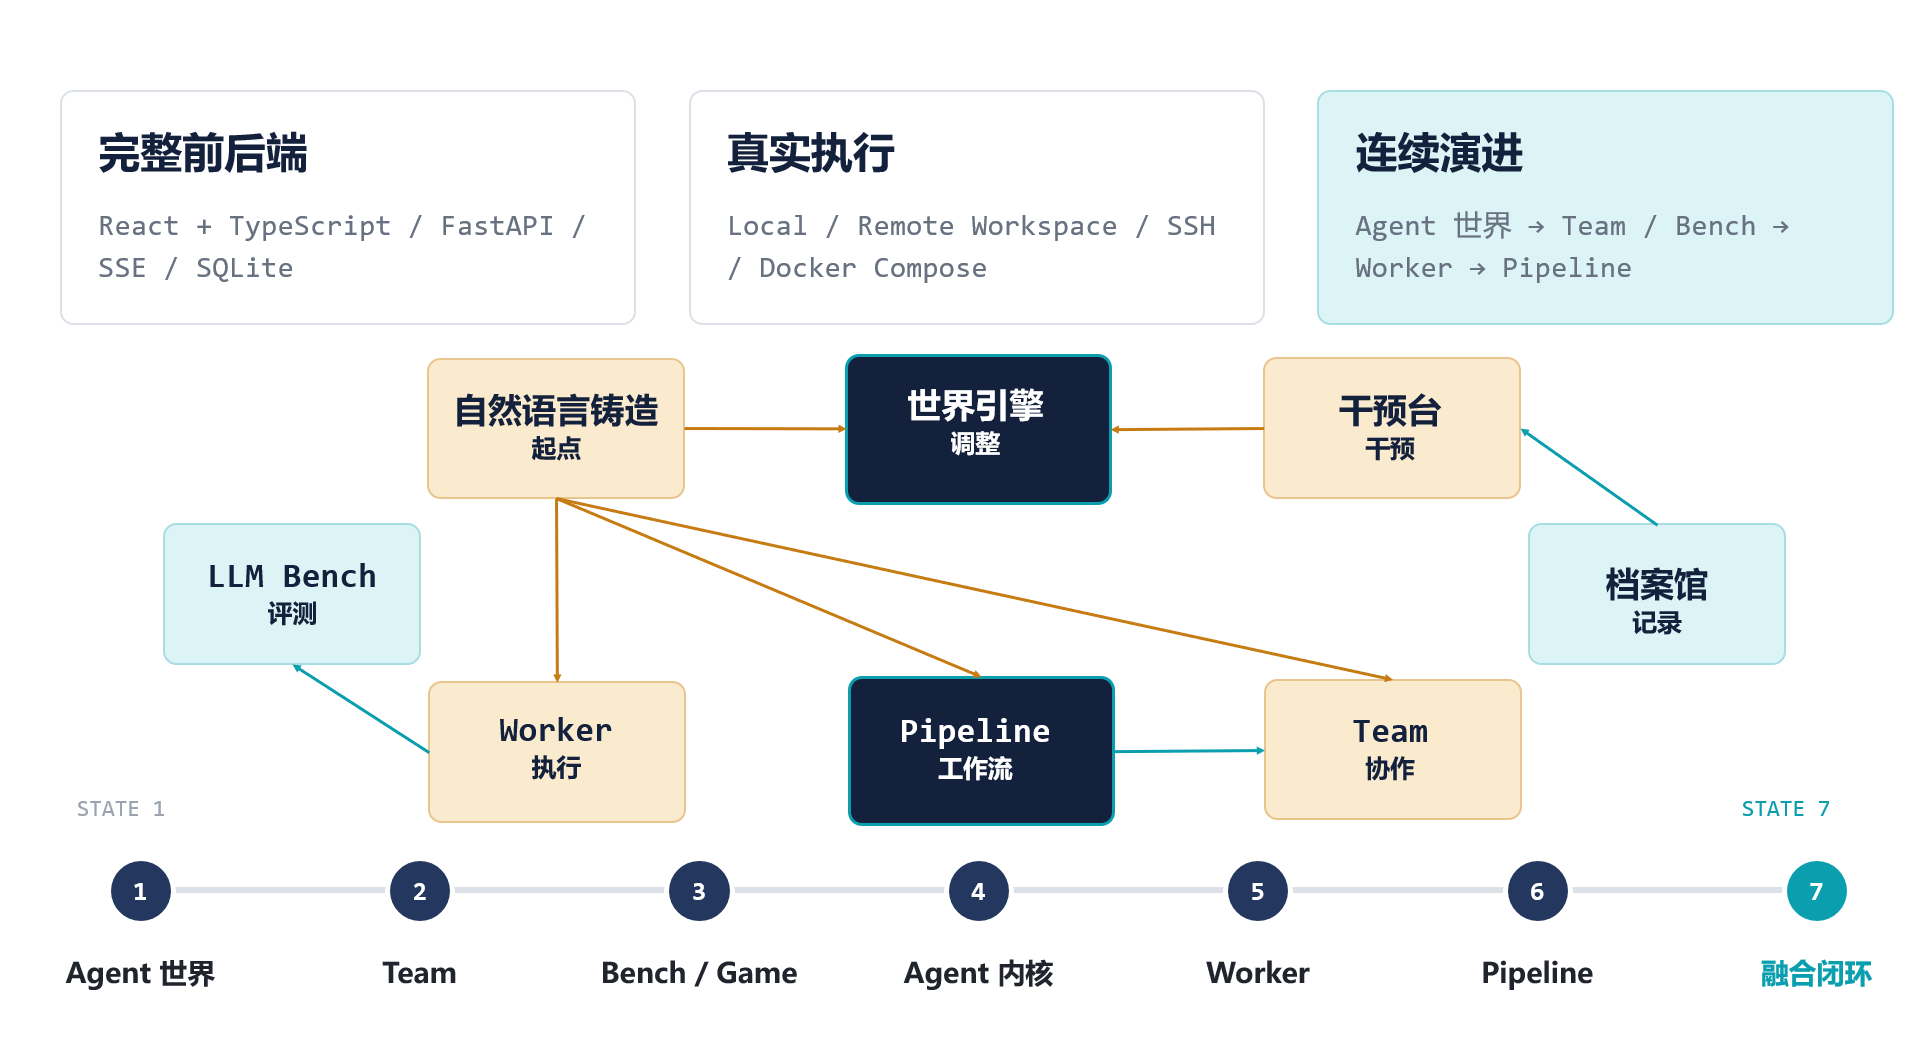
\includegraphics[width=0.95\textwidth]{arch_circle.png}
	\caption{Life Lab 七阶段连续演进：从 Agent 世界（STATE 1）到融合闭环（STATE 7），涵盖完整前后端、真实执行、LLM Bench、Pipeline 工作流等核心能力。}
	\label{fig:lifecycle}
\end{figure}


%% ============================================================
\section{基础模块设计（M1--M8）}
%% ============================================================

基础模块覆盖 Agent 从"诞生"到"沉淀"的完整生命周期，为进阶能力提供不可或缺的人格基底和行为数据。

\subsection{人格数据模型（M1）}

\begin{table}[H]
	\centering
	\begin{tabular}{cll}
		\toprule
		\textbf{组件} & \textbf{类型} & \textbf{说明} \\
		\midrule
		MBTI & string & 16 种人格类型 + T/A 变体 \\
		BigFive & struct & 五维浮点参数 (0--1)：开放性、尽责性、外向性、宜人性、神经质 \\
		DecisionStyle & struct & 四维决策风格：信息处理、风险偏好、社交倾向、压力应对 \\
		Values & list[string] & 核心价值观列表 \\
		Narrative & string & 200--400 字人格画像 \\
		Background & struct & 背景故事（家乡、家庭、教育、关键事件） \\
		Goals & list[Goal] & 层级化目标（优先级 + 截止日期 + 进度） \\
		EmotionalState & struct & VAD 三维情绪模型（愉悦度、唤醒度、支配感） \\
		\bottomrule
	\end{tabular}
\end{table}

PersonaBuilder 接收自然语言描述，通过 LLM 生成完整人格 JSON。System Message 采用"冻结核心 + 动态上下文"双层结构：核心层（身份、价值观、目标）初始化后不变，上下文层（处境、记忆、笔记）每 tick 注入，确保人格一致性与环境感知的平衡。

\subsection{世界引擎与关系双轨评估（M2/M3）}

世界引擎采用离散时间模拟（Tick-Based），每个 tick 顺序执行：构建上下文、注入 Agent、执行决策、后处理（Tool 副作用、目标更新、关系演化）、推送 SSE 事件。

Agent 之间的关系不是简单的“好友/敌人”二分，而是一个 $[-1, +1]$ 的连续分数。分数的更新采用两条路径协同工作：
\begin{itemize}
	\item \textbf{快速路径}（每 tick）：检测对话中的关键词（如“谢谢”“讨厌”“一起”），匹配 7 种交互类型，即时更新关系分数。1ms 内完成，保证每 tick 都有反馈。
	\item \textbf{深度路径}（每 3 tick，异步）：让 LLM 阅读全部事件，评估关系变化。能捕捉关键词无法识别的微妙情感（如反讽、暗示），但需要数秒。
\end{itemize}
快速路径保证实时性，深度路径补充准确性，两者协同使关系演化既实时又准确。

7 种交互类型及其对关系分数的影响：

\begin{table}[H]
	\centering
	\begin{tabular}{clp{5.5cm}}
		\toprule
		\textbf{类型} & \textbf{$\Delta$} & \textbf{典型关键词} \\
		\midrule
		友好 (friendly) & $+0.10$ & 谢谢、喜欢、欣赏、支持 \\
		敌对 (hostile) & $-0.15$ & 讨厌、滚、闭嘴、嘲讽 \\
		合作 (cooperative) & $+0.08$ & 一起、合作、讨论、分享 \\
		竞争 (competitive) & $-0.05$ & 比、赢、挑战、超过 \\
		支持 (supportive) & $+0.12$ & 我相信你、别担心、有我在 \\
		轻视 (dismissive) & $-0.10$ & 随便、无所谓、别烦我 \\
		好奇 (curious) & $+0.05$ & 为什么、你怎么看、然后呢 \\
		\bottomrule
	\end{tabular}
\end{table}

关系分数在 $[-1, +1]$ 区间内累积演化，A$\to$B 和 B$\to$A 独立计算，确保同一对 Agent 可以存在不对称关系。快速路径保证每 tick 都有关系更新，深度路径补充微妙的情感信号，两者协同使关系演化既实时又准确。

\subsection{叙事、竞技与干预（M4--M8）}

\textbf{竞技引擎}（M4）支持辩论、面试、路演、盲测和大乱斗五种模式。辩论模式采用逐阶段淘汰制，面试模式模拟真实群面流程，盲测模式隐藏 Agent 身份避免偏见，裁判从逻辑性、创造性、表达力、人格一致性四维度评分。

\textbf{叙事引擎}（M5）将 Agent 经历转化为 9 种文体叙事（小说/日记/信件/播客脚本等），保持 Agent 口吻一致。每种文体有独立的 Prompt 模板，LLM 不可用时自动降级为基于事件序列的规则兜底。

\textbf{控制台}（M6）提供上帝视角仪表盘和决策模式识别，自动统计 Agent 的分析型/直觉型/果断型/谨慎型占比并实时可视化，帮助用户理解不同人格的决策倾向。

\textbf{干预台}（M7）支持运行时注入公共事件（影响全体 Agent）和私密指令（仅目标 Agent 可见），实现上帝视角的社会实验控制——研究者可以在不中断模拟的前提下观察特定干预对 Agent 行为的影响。

\textbf{档案馆}（M8）支持实验完整回放（逐 tick 事件序列）、模板沉淀（将成功的 Agent 配置保存为可复用模板）和报告导出，确保每次实验都可追溯、可复现。

%% ============================================================
%% 以下为进阶模块（M9--M12），是本平台的技术深度所在
%% ============================================================

\newpage
\section{团队协作引擎（M9）}
%% ============================================================

M9 实现完整的多 Agent 协作工作流。以一个 3 人团队执行"撰写市场调研报告"为例：LLM 将任务分解为"资料搜集""数据分析""报告撰写"三步，分别分配给研究型、分析型和写作型 Agent。三步形成线性 DAG（搜集$\to$分析$\to$撰写），同层最多 3 路并行（本例中每层仅 1 个节点）。Agent A 完成资料搜集后，产出文件自动复制到 Agent B 的工作区；Agent B 基于真实文件（而非 Agent A 的"口头描述"）进行分析。交付验收时，程序检查 Agent B 是否真正调用了 read\_file 工具读取了 Agent A 的产出，而非凭空生成分析结果。以下聚焦三个核心设计决策。

\subsection{设计决策一：文件系统 与 消息通信}

\textbf{方案}：Agent 间通过共享文件系统协作，而非消息队列或 API 调用。

\textbf{理由}：文件系统天然具备\textbf{可追溯性}（所有协作留痕）、\textbf{可调试性}（随时查看任意步骤的输入输出）和\textbf{可回放性}（实验可完整复现）。每步工作区自动复制上游成功步骤的产出文件给下游，确保信息传递不依赖 Agent 的"记忆"。

\textbf{隔离规则}：Team 工作区与 Worker 工作区位于不同父目录，互不干扰。Team 工作区包含共享任务描述（TASK.md）、团队配置（TEAM.json）和每步骤的上下文文件。

\subsection{设计决策二：LLM 分解 + 规则兜底}

\textbf{方案}：任务分解优先使用 LLM，LLM 不可用时降级为基于角色的规则分配（8 种预设角色模板）。

\textbf{理由}：LLM 分解灵活但不可靠（可能返回不存在的 Agent 名字），规则分解可靠但死板。两者结合既保证了正常路径的智能性，又保证了降级路径的可用性。安全网机制自动将 LLM 返回的名字映射为合法 UUID。

\textbf{角色演化}：每个步骤成功后，LLM 作为"团队观察者"评估 Agent 实际表现并动态调整其角色描述，使团队分工在执行中自我优化。

\subsection{设计决策三：团队诊断与容错}

\textbf{团队诊断}：DiagnosticsEngine 实时监控参与度（静默过久触发告警）、参与度评分（基于发言占比）和冲突检测（同一 tick 内过多并行操作时标记）。

\textbf{容错机制}：步骤失败时，保留已完成上下文，仅对剩余步骤重新分解，避免从零开始。Worker 内部具备 JSON 解析重试和 LLM 调用指数退避机制。

%% ============================================================
\section{评测基准（M10）}
%% ============================================================

M10 的设计核心是\textbf{可解释的行为分析}，即：不仅给分，还要解释"为什么"。

\subsection{设计决策一：鲁棒性为什么是跨任务指标}

\textbf{问题}：单次任务中的"鲁棒性"无法衡量、LLM存在随机性，一个 Agent 在一次模拟中可能碰巧表现很好。

\textbf{方案}：单任务中的鲁棒性只是占位值。通过一个 Agent 在多次任务中得分是否稳定评估。用统计中的\textbf{变异系数}（Coefficient of Variation）来衡量。设 $n$ 次评测的分数为 $s_1, s_2, \ldots, s_n$，定义：
\[
\mu = \frac{1}{n}\sum_{i=1}^{n}s_i, \quad \sigma = \sqrt{\frac{1}{n}\sum_{i=1}^{n}(s_i - \mu)^2}, \quad cv = \frac{\sigma}{\mu}
\]
则鲁棒性指标为：
\[
R = \max(0,\; 100 - cv \times 100)
\]
当所有任务分数完全一致时 $cv = 0$，$R = 100$（满分）；分数波动越大，$cv$ 越大，$R$ 越低。

\textbf{设计考量}：失败任务的零分也进入聚合，避免只统计成功样本导致结果虚高。例如，某 Agent 在 3 次评测中得分为 80、82、78，则 $\mu = 80$，$\sigma \approx 1.63$，$cv \approx 0.02$，$R \approx 98$，则表现极其稳定。

\subsection{设计决策二：行为指纹为什么用信息熵}

\textbf{问题}：如何量化"Agent 的行为是否一致"？简单的统计量（如平均值）无法捕捉行为分布的特征。

\textbf{方案}：思路很直接：统计 Agent 使用了哪些工具、各用了多少次。如果总是用同一种工具，说明行为很聚焦；如果均匀地使用各种工具，说明行为很分散。用 Shannon 信息熵（Shannon, 1948）把这个直觉变成公式。设 Agent 在 $T$ 个 tick 内共调用 $N$ 次工具，各工具调用频率为 $n_1, n_2, \ldots, n_k$（$\sum n_i = N$），定义概率分布 $p(x_i) = n_i / N$：
\[
H(X) = -\sum_{i=1}^{k} p(x_i) \log_2 p(x_i)
\]
最大熵 $H_{\max} = \log_2 k$（均匀分布时取到）。定义\textbf{行为一致性分数}：
\[
C = 1 - \frac{H(X)}{H_{\max}}
\]
$C \in [0, 1]$：$C \to 1$ 表示行为高度聚焦（几乎只用一种工具），$C \to 0$ 表示行为高度分散（均匀使用所有工具）。

\textbf{具体示例}：Agent A 在 10 次调用中全部使用同一工具（observe），则 $H = 0$，$C = 1.0$，行为高度聚焦，为"观察型"Agent。Agent B 均匀调用 3 种工具各 3--4 次，则 $H \approx 1.585 = H_{\max}$，$C \approx 0.0$，行为高度分散，为"多面手"Agent。信息熵有效区分了两种截然不同的行为模式。

\subsection{设计决策二-b：决策风格如何量化分类}

\textbf{问题}：一致性分数 $C$ 只能衡量行为的聚焦/分散程度，无法区分"聚焦于什么"。

\textbf{方案}：从 Agent 的动作关键词中提取四类决策风格并量化占比。设 Agent 的动作关键词集合为 $A$，四类关键词集分别为：
\begin{itemize}
	\item \textbf{分析型} $K_\alpha$：分析、判断、计划
	\item \textbf{直觉型} $K_\beta$：想要、尝试、选择
	\item \textbf{果断型} $K_\gamma$：决定、坚持、接受
	\item \textbf{谨慎型} $K_\delta$：避免、拒绝、妥协
\end{itemize}
各风格占比定义为 $\alpha = |\{a \in A : a \in K_\alpha\}| / |A|$，$\beta$、$\gamma$、$\delta$ 同理。当某一类占比 $> 30\%$ 时归为对应风格（可叠加，如"分析型+果断型"），否则为"平衡型"。配合逐维度诊断证据链（思考次数、消息长度、回复标准差等），评测结果完全可解释。

\subsection{设计决策三：诊断评分的设计动机}

\textbf{问题}：传统评测只给分数。用户无法判断这个分数是否合理。

\textbf{方案}：诊断评分从原始事件证据中逐维度追溯评分原因。例如"思考次数偏少(5次)，内部推理不充分"或"回复长度标准差: 42，能根据情境调整表达方式"。配合劣化趋势检测（对比最近 3 次与前 3 次评测），可以看到完整的证据链。

%% ============================================================
\section{游戏化场景（M11）}
%% ============================================================

M11 的核心创新是\textbf{MBTI 人格到游戏行为的端到端映射}，通过构建随机引擎，实现人格不仅影响"说什么"，还影响"怎么走"和"如何感受"。

\subsection{设计决策一：MBTI 到行为的映射}

\textbf{选择}：MBTI 直接推导移动参数（间隔、范围、空闲率），而非通过 prompt 间接影响。

\textbf{映射规则}：E/I 维度决定活动频率（外向型移动间隔短），T/F 维度决定行为倾向，N/S 维度决定探索范围。4 种人格组合各有独立的移动配置：

\begin{table}[H]
	\centering
	\begin{tabular}{lccc}
		\toprule
		\textbf{人格组合} & \textbf{移动间隔(ms)} & \textbf{最大范围(格)} & \textbf{空闲概率} \\
		\midrule
		内向思考型（I\_T\_） & 9000--16000 & 2 & 0.45 \\
		内向感受型（I\_F\_） & 7000--13000 & 2 & 0.35 \\
		外向思考型（E\_T\_） & 4000--9000 & 3 & 0.15 \\
		外向感受型（E\_F\_） & 3500--8000 & 3 & 0.10 \\
		\bottomrule
	\end{tabular}
\end{table}

\textbf{混合策略}：移动目标选择采用物品寻求 + 社交接近 + 随机漫游的混合策略，使 Agent 的行为既有目的性又有随机性。

\subsection{设计决策二：情绪引擎的多重触发}

\textbf{选择}：EmotionEngine 集成五重触发链，而非单一的情绪模型。

\begin{itemize}
	\item \textbf{对话触发}：关键词规则匹配 8 种情绪，对话气泡弹出时即时分析。
	\item \textbf{环境触发}：场景氛围（6 种场景各有情绪偏向）+ 邻近物品情绪影响。
	\item \textbf{社交共鸣}：近距离同情绪 Agent 互相放大，异情绪互相中和。
	\item \textbf{随机事件}：场景事件池（6 种场景共 25+ 事件）定期触发。
	\item \textbf{衰减回归}：情绪强度自然向中性回归。
\end{itemize}

\textbf{理由}：单一触发（如只有对话触发）不够真实。真实的情绪受多种因素共同影响，例如对话内容、所处环境、社交对象、突发事件和自然消退。五重触发链使 Agent 的情绪变化更加自然和可观察。

场景氛围与物品情绪的具体设计：

\begin{table}[H]
	\centering
	\begin{tabular}{clcl}
		\toprule
		\textbf{场景} & \textbf{氛围情绪} & \textbf{物品} & \textbf{情绪影响} \\
		\midrule
		图书馆 & 中性 & 床/沙发 & 疲倦 \\
		宿舍 & 疲倦 & 钢琴/喷泉 & 愉悦 \\
		教室 & 焦虑 & 自动售货机 & 兴奋 \\
		艺术中心 & 愉悦 & 电脑 & 困惑 \\
		实验室 & 困惑 & 地球仪 & 惊讶 \\
		樱花大道 & 愉悦(\texttimes 2) & 树/盆栽 & 愉悦/中性 \\
		\bottomrule
	\end{tabular}
\end{table}

系统还维护了 25+ 条场景随机事件（如"图书馆突然停电""实验数据突然对上了""花瓣纷纷飘落"等），每 30--70s 随机触发一条，影响全体或随机个体。情绪引擎通过三条独立定时器协同工作：衰减定时器（每 30s 情绪向中性回归一级）、环境定时器（每 30s 场景与物品情绪微调）、随机事件定时器（30--70s 间隔），使 Agent 的情绪变化具有真实的时间节律。

\subsection{设计决策三：目标预订防碰撞协议}

\textbf{选择}：借鉴分布式系统的资源预订协议（Reserve-Move-Release 三步），而非简单的碰撞检测。

\textbf{理由}：碰撞检测是"事后补救"（碰撞发生后再处理），目标预订是"事前预防"（移动前先确认目标格可用）。这确保了即使在高并发场景下，Agent 的空间行为也是\textbf{确定性的}，保障同一格不会被分配给两个 Agent。

%% ============================================================
\section{管道编排引擎（M12）}
%% ============================================================

M12 的核心是一个支持复杂控制流的 DAG 管道编排引擎。

Worker 是管道中的执行单元，每个 Worker 通过显式状态机管理任务生命周期，共 6 个正常状态：IDLE（等待任务）$\to$ PLANNING（制定执行计划）$\to$ DECIDING（决策下一步）$\to$ EXECUTING（执行工具调用）$\to$ REFLECTING（反思结果）$\to$ DONE（完成）。反思阶段可回到 DECIDING（继续）、PLANNING（修订计划）或直接到 DONE。系统设有最大步数限制防止无限循环。错误处理采用三级策略：RETRYABLE（网络超时等，自动重试）、SKIPPABLE（文件缺失等，Agent 自主决策）、FATAL（API 连续失败等，立即终止）。特别地，REFLECTING $\to$ PLANNING 的"修订"路径使 Worker 能根据交付验收反馈自动调整计划并重新执行，形成"执行$\to$验收$\to$修订"的闭环迭代。

\subsection{设计决策一：Loop/Branch的设计动机}

\textbf{问题}：简单 DAG 只能表达"一次性"执行。现实中很多工作流需要迭代（"分析 $\to$ 评审 $\to$ 不合格则修改"）和条件跳转（"如果搜索到足够信息则跳过补充搜索"）。

\textbf{方案}：在标准 DAG 的 FLOW 边之外，增加 LOOP（回边循环）和 BRANCH（条件跳转）两种边类型。条件值从节点\textbf{真实产出文件}中读取，支持正则匹配、数值比较和关键词检测三种模式。

\textbf{执行策略}：拓扑排序后按层级执行，同层节点最多 3 路并行。Loop 触发时将回边路径上的节点重新入队，Branch 触发时 BFS 标记被绕过节点为跳过。

\subsection{设计决策二：确定性硬校验的设计动机}

\textbf{问题}：LLM 验收员本身也可能产生"幻觉"，它可能误判一个有算式错误的交付为"通过"。这是 LLM 系统的固有风险。

\textbf{方案}：在 LLM 验收之前，先让程序自己检查，而不是让 LLM 去“看”算式对不对（可能看错），不如直接让程序算一遍。具体有两道检查：
\begin{enumerate}
	\item \textbf{算式 AST 求值}：对交付物中的数学表达式，解析为抽象语法树（AST）后直接求值，判断计算是否正确。例如 "$3 + 5 \times 2$" 解析为 $\mathrm{Add}(3,\, \mathrm{Mul}(5, 2))$，求值得 $13$，与交付结果比对。
	\item \textbf{工具台账核验}：检查 Agent 声称执行的工具调用是否在机器台账中有真实记录，查验工具名是否存在、参数是否合法、返回值是否已写入产出文件。
\end{enumerate}
硬校验发现的问题\textbf{强制标记为失败}，即使 LLM 验收员误判也无法绕过。

\textbf{设计考量}：确定性规则（快速硬校验，$O(1)$ 判断）与 LLM 判断（慢速语义评估）互相保险。其核心洞察是：\textbf{用确定性对抗随机性}，规则校验不会"幻觉"，而 LLM 判断可能"幻觉"，两条独立路径防止同源错误。

\subsection{设计决策三：自动修订机制}

\textbf{选择}：首次验收不通过时，将问题反馈送回 Worker 自动修订，最多两轮复验。

\textbf{理由}：验收不视作终点，而是迭代的一部分。自动修订使 Agent 有机会纠正错误，而不是简单地标记失败。超过修订上限后，当前工作区保留，用户可手动补充。

%% ============================================================
\section{平台运行评测数据}
%% ============================================================

平台在实际运行中积累了完整的评测数据，所有数据存储于 SQLite 数据库（\texttt{lifelab.db}），以下数据均从数据库中直接提取。

\subsection{评测数据总览}

\begin{table}[H]
	\centering
	\begin{tabular}{lc}
		\toprule
		\textbf{数据类型} & \textbf{记录数} \\
		\midrule
		Bench 完整评测运行 & 4 次（全部完成，27/27 任务） \\
		Bench 子结果 & 94 条 \\
		Arena 竞技对抗 & 1 场（6 人大乱斗） \\
		Team 团队协作 & 5 个团队，14 个计划 \\
		Agent 实例 & 25 个 \\
		World 世界实例 & 48 个 \\
		Simulation 模拟运行 & 47 次 \\
		\bottomrule
	\end{tabular}
\end{table}

4 次 Bench 评测均使用 deepseek-v4-flash 模型，采用标准评测套件（3 Agent $\times$ 3 场景 $\times$ 3 重复 = 27 条评测记录/次）。标准 Agent 为学霸小明（INTJ-T）、社交小红（ENFP-A）、领导者小刚（ESTJ-A），标准场景为期末周、新生报到、毕业选择。

\subsection{六维雷达评测结果}

每次评测从人格一致性、决策质量、交互深度、鲁棒性、创造力、适应性六个维度（每维 0--100 分）对 Agent 行为进行量化评分。4 次运行的评分如下：

\begin{table}[H]
	\centering
	\small
	\begin{tabular}{lcccccc}
		\toprule
		\textbf{维度} & \textbf{运行 1} & \textbf{运行 2} & \textbf{运行 3} & \textbf{运行 4} & \textbf{平均} \\
		\midrule
		人格一致性 & 32.6 & 31.2 & 35.1 & 32.6 & 32.9 \\
		决策质量 & 32.8 & 33.8 & 37.4 & 35.6 & 34.9 \\
		交互深度 & 32.6 & 34.3 & 35.7 & 33.7 & 34.1 \\
		鲁棒性 & 92.6 & 92.4 & 92.0 & 94.1 & 92.8 \\
		创造力 & 57.8 & 57.2 & 54.1 & 57.4 & 56.6 \\
		适应性 & 89.3 & 87.0 & 86.6 & 92.3 & 88.8 \\
		\bottomrule
	\end{tabular}
\end{table}

其中鲁棒性使用变异系数计算：$cv = \sigma/\mu$，$R = \max(0, 100 - cv \times 100)$，即 Agent 在多次重复评测中得分越稳定，鲁棒性越高。

\subsection{分 Agent 与分场景聚合}

下表展示各 Agent 在不同场景下的平均评分（跨 4 次运行聚合）：

\begin{table}[H]
	\centering
	\small
	\begin{tabular}{llcccccc}
		\toprule
		\textbf{Agent} & \textbf{场景} & \textbf{人格} & \textbf{决策} & \textbf{交互} & \textbf{鲁棒} & \textbf{创造} & \textbf{适应} \\
		\midrule
		学霸小明 & 期末周 & 45.8 & 30.0 & 28.4 & 80.0 & 66.0 & 91.7 \\
		学霸小明 & 新生报到 & 33.1 & 30.0 & 26.8 & 80.0 & 58.8 & 97.7 \\
		学霸小明 & 毕业选择 & 31.0 & 34.2 & 34.5 & 80.0 & 55.1 & 88.6 \\
		\midrule
		社交小红 & 毕业选择 & 38.2 & 33.1 & 30.2 & 80.0 & 57.5 & 81.1 \\
		社交小红 & 期末周 & 30.0 & 36.2 & 36.1 & 80.0 & 52.0 & 85.8 \\
		社交小红 & 新生报到 & 30.0 & 33.1 & 22.2 & 80.0 & 53.5 & 90.8 \\
		\midrule
		领导者小刚 & 毕业选择 & 30.0 & 55.0 & 66.4 & 80.0 & 49.3 & 100.0 \\
		领导者小刚 & 期末周 & 30.0 & 30.3 & 32.7 & 80.0 & 57.0 & 86.0 \\
		领导者小刚 & 新生报到 & 30.0 & 33.6 & 40.1 & 80.0 & 53.1 & 78.4 \\
		\bottomrule
	\end{tabular}
\end{table}

\subsection{Arena 竞技对抗记录}

平台记录了 1 场 6 人 Arena 大乱斗（创业路演主题：有限校园创新基金应该交给谁使用），采用逐阶段淘汰制，LLM 裁判从逻辑性、创造性、表达力、人格一致性四维度评分。最终林启明获得冠军，慧兰获得亚军。比赛经历 3 个阶段、42 轮发言，完整记录了每位参赛者的思维链（think\_aloud）和对话内容。

\subsection{团队协作运行统计}

5 个团队共执行 14 个计划，验证了以下核心特性：
\begin{itemize}
	\item 任务分解：LLM 分解失败时自动降级为规则分配
	\item 执行幂等性：重复执行不会创建重复记录
	\item 交付硬校验：算式 AST 求值 + 工具台账核验（程序直接验证，不依赖 LLM）
\end{itemize}

\subsection{评测结果分析}

\begin{enumerate}
	\item \textbf{鲁棒性最强}（平均 92.8 分）：模型在跨场景、跨重复运行中表现高度稳定，输出一致性好。
	\item \textbf{人格一致性最弱}（平均 32.9 分）：Agent 行为未能严格遵循 MBTI 设定，人格参数对行为的约束力不足，是后续优化的核心方向。
	\item \textbf{不同 Agent 在不同场景下表现差异明显}：学霸小明在期末周（高压学术场景）人格一致性最高（45.8），领导者小刚在毕业选择场景交互深度最高（66.4），体现了人格与场景的耦合效应。
	\item \textbf{适应性维度波动较大}（78.4--97.7）：学霸小明在新生报到场景适应性最强（97.7），领导者小刚在新生报到场景最弱（78.4），说明不同人格对环境变化的响应模式存在显著差异。
\end{enumerate}

%% ============================================================
\section{大模型应用与调试优化}
%% ============================================================

\subsection{模型接入与调用方式}

Life Lab 通过 OpenAI 兼容 API 统一接入多种大语言模型，评测中使用 \textbf{DeepSeek-V4-Flash}（api.deepseek.com），同时支持 GLM、OpenAI 等模型的无缝切换。

\begin{itemize}
	\item \textbf{双模式配置}：系统为不同场景配置了"思考"（think）和"行动"（act）两种 LLM 配置。思考模式使用较高温度用于深度推理（如人格铸造、关系评估），行动模式使用较低温度用于快速决策（如工具调用、动作选择）。
	\item \textbf{Prompt 工程}：System Message 采用"冻结核心 + 动态上下文"双层结构，核心层（身份、价值观、目标）初始化后不变，上下文层（处境、记忆、笔记）每 tick 注入，确保人格一致性与环境感知的平衡。
	\item \textbf{联网搜索}：集成 DeepSeek Responses API 内置联网搜索，并配备搜狗/百度/Bing 多引擎并行兜底，支持断路器保护避免连续失败。
\end{itemize}

Worker 决策 Prompt 的设计遵循一个关键约束：\textbf{Agent 输出必须是严格 JSON，不包含额外文字}。这是从 Team 模式（GroupChat）中吸取的教训——自由文本发言导致解析不可控。系统从不在 Prompt 中暴露 JSON Schema 语法（模型容易混淆 \texttt{"a" | "b"} 这类写法），而是通过具体示例引导格式。当 JSON 解析失败时，系统追加格式提示（含完整示例），最多 3 次重试。

\subsection{调试与优化策略}

针对 LLM 系统的固有不稳定性，平台实现了多层次的调试与优化机制：

\begin{itemize}
	\item \textbf{超时重试与指数退避}：所有 LLM 调用包装在统一的异步调用器中，默认超时取 settings.agent\_timeout\_seconds，重试间隔采用指数退避（2s、4s、8s），避免对 API 服务造成压力。
	\item \textbf{断路器保护}：联网搜索模块实现断路器机制，连续失败达到阈值后自动断开，避免反复超时拖慢系统。
	\item \textbf{统一错误分类}：通过 LLMErrorClassifier 将上游 OpenAI 兼容异常（AuthenticationError、RateLimitError、TimeoutError、ConnectionError）转换为用户友好的中文提示，方便定位问题。
	\item \textbf{LLM 不可用降级}：任务分解、关系评估等关键路径均有规则兜底方案，LLM 不可用时自动降级为基于关键词/角色的规则引擎，确保系统在任何环境下可用。
	\item \textbf{JSON 解析重试}：Worker 内部对 LLM 返回的 JSON 进行解析重试，处理格式不规范的情况。
	\item \textbf{LLM 幻觉交付发现与解决}：在早期测试中，Worker Agent 在交付阶段声称"已完成数据分析"，但实际从未调用过 run\_python 或 read\_file 工具——LLM 验收员竟然也判定为"通过"。这暴露了纯 LLM 验收的根本风险：\textbf{执行者和验收者可能犯同一类错误}。由此引入了程序级硬校验：在 LLM 验收之前，先让程序检查工具台账（Agent 是否真的调用过相关工具）和算式 AST 求值（交付物中的数学表达式是否正确）。硬校验结果强制生效，LLM 无法覆盖。
	\item \textbf{评测趋势监控}：BenchLab 自动检测评测分数连续下降趋势（对比最近 3 次评测），及时提醒用户可能存在的模型退化问题。
\end{itemize}

%% ============================================================
\section{系统实现与前端}
%% ============================================================

前端采用 React 18 + TypeScript + Vite，通过 React Query 管理服务端状态、Zustand 管理客户端状态、SSE 实现实时通信，Phaser 3 渲染游戏化场景，Recharts 绘制评测图表。系统共实现 \textbf{20+ 页面}，覆盖 12 个模块的全部功能：

\begin{table}[H]
	\centering
	\small
	\begin{tabular}{clp{6cm}}
		\toprule
		\textbf{模块} & \textbf{页面} & \textbf{功能描述} \\
		\midrule
		通用 & Home, GuidePage, Settings & 首页、功能引导、设置 \\
		M1 & AgentFoundry, AgentModule & 人格铸造、Agent 管理 \\
		M2/M3 & SoloTheater, GroupSandbox, GameScene & 单人/群体场景、游戏渲染 \\
		M4 & Arena, DuelArena & 竞技场、对决 \\
		M5 & NarrativeFactory & 叙事生成 \\
		M6/M7 & ControlPanel, DirectorIntervention & 控制台、干预 \\
		M8 & Archive, ShowcaseWall & 档案、展示 \\
		M9 & TeamDashboard & 团队监控 \\
		M10 & BenchLab & 评测实验 \\
		M12 & WorkerBench, PipelinePage, PipelineEditor & Worker、管线管理、图形化编辑器 \\
		\bottomrule
	\end{tabular}
\end{table}

数据层通过 Pydantic 模型 + SQLAlchemy 异步 ORM + aiosqlite 实现全异步操作，核心表包括 AgentRow（人格 JSON、情绪状态、指纹 JSON）、WorldRow、TeamRow、PlanRow、BenchRun、BenchResult、MemoryRow 共 7 张。

前端技术亮点包括：(1) SSE 驱动的实时事件流——Agent 的每次思考（think\_aloud）、每次工具调用、每次情绪变化都通过 Server-Sent Events 毫秒级推送到前端，实现"思维流"可视化；(2) Phaser 3 游戏化渲染——2D 瓦片地图上的 Agent 精灵支持 5 种动作状态（idle/walk/talk/think/emote），情绪状态通过头顶气泡实时反馈；(3) 图形化管线编辑器——基于 React Flow 构建，支持拖拽创建 DAG 节点、配置 Loop/Branch 控制流、实时查看每个节点的执行状态。

%% ============================================================
\section{总结}
%% ============================================================

Life Lab 要解决三个工程问题：LLM 会幻觉——Agent 声称完成了任务却从未执行；行为会同质化——不同人格的 Agent 在场景中表现几乎相同；评测是黑箱——只给分数不给原因。

针对交付幻觉，Life Lab 的回答是\textbf{程序级校验}：算式直接算一遍，工具记录直接查一遍，硬校验结果强制生效，LLM 验收员误判也无法绕过。针对行为同质化，Life Lab 的回答是\textbf{信息论量化}：用 Shannon 信息熵把"人格是否影响行为"从主观判断变为可计算的数学命题。针对评测黑箱，Life Lab 的回答是\textbf{逐维度诊断}：每个分数都有完整证据链，可以看到"为什么得了这个分"。

贯穿这三个回答的核心工程洞察是\textbf{用确定性对抗随机性}：关键词检测保证实时性，LLM 深度评估保证准确性，程序级校验防止 LLM 判断出错，超时重试/断路器/降级兜底保证系统可用性。这一模式在关系评估、任务分解、交付验收中反复出现，是平台的核心工程哲学。

七个阶段、12 个模块、25 个 Agent、94 条评测子结果、鲁棒性 92.8 分——Life Lab 不是一个仅能演示的玩具，而是一个可以真正用来探索 AI 社会性行为的实验平台。人格可以被铸造，行为可以被观测，涌现可以被量化，协作可以被信赖。

\end{document}
